\documentclass[11pt]{article}
\usepackage[margin=1.0in]{geometry}
\usepackage{ragged2e}
\usepackage{amsmath}    % Expanded math operations for papers
\usepackage{amssymb}
%\usepackage{esvect}    % Vector notation for mathematics
\usepackage{graphicx}
\usepackage{wrapfig}    % Format figures more appropriately
\usepackage{hyperref}   % Enable hyperlink support
\usepackage{fancyhdr}   % Allow headers and footers customized
\usepackage{titlesec}   % Allow customization of section headers
\usepackage{wrapfig}    % So I can wrap figures around my text
\usepackage{enumitem}	% Align things in the itemize environment
\usepackage{subcaption}
\usepackage[font=small,skip=0pt]{caption}

% Set up code environment
\usepackage{listings}
\usepackage{color}

\definecolor{mygreen}{RGB}{28,172,0} % color values Red, Green, Blue
\definecolor{mylilas}{RGB}{170,55,241}

\lstset{language=Matlab,%
    %basicstyle=\color{red},
    breaklines=true,%
    morekeywords={matlab2tikz},
    keywordstyle=\color{blue},%
    morekeywords=[2]{1}, keywordstyle=[2]{\color{black}},
    identifierstyle=\color{black},%
    stringstyle=\color{mylilas},
    commentstyle=\color{mygreen},%
    showstringspaces=false,%without this there will be a symbol in the places where there is a space
    numbers=left,%
    numberstyle={\tiny \color{black}},% size of the numbers
    numbersep=9pt, % this defines how far the numbers are from the text
    emph=[1]{for,end,break},emphstyle=[1]\color{red}, %some words to emphasise
    %emph=[2]{word1,word2}, emphstyle=[2]{style},    
}

% Set graphics path
\graphicspath{ {Figures/} }

% Reformat section headers
\titleformat{\section}{\normalfont\large\bfseries}{\thesection}{1em}{}[{\titlerule[0.8pt]}]
\titleformat{\subsection}{\normalfont\large\bfseries}{\thesubsection}{1em}{}
\titleformat{\subsubsection}{\normalfont\normalsize\bfseries}{\thesubsubsection}{1em}{}

% Define page header and footer
\pagestyle{fancy}
\fancyhf{}
\lhead{Seaborn • Buchanan • Sambolu}
\rhead{March 26, 2019}
\lfoot{ECE 460}
\rfoot{Page \thepage}


\begin{document}



%
%%---------------------------------------------------------------------------------------------------| TITLE
%

\begin{Large}\begin{center}
Custom Audio Equalizer
\end{center}\end{Large}


%
%%---------------------------------------------------------------------------------------------------| PROJECT APPROACH
%

\section{Project Approach}

\noindent We studied professional audio equalizers and research how they are used in the industry to seek inspiration for our approach to the equalizer software. Alice consulted his friend, a music major at Bradley, on what frequency ranges were typically used to isolate different musical components.

\begin{figure}[h!]
	\begin{quote}
	The typical ranges for Eqs would be roughly: Low is 20hz- 400hz, Mids would be 500hz -3000hz, and highs from 4000hz - 20,000hz. There’s defiantly some blend from range to range but these are generally where they sit. Also once you hit 1000hz changes in sound quality become farther spread out(meaning 1000-2000hz becomes as noticeable as 100-300hz). I hope that makes sense.
	\end{quote}
	\caption{Assistance in determining ideal equalizer bands.}
\end{figure}

With more research we verified Kuda's advice and used 20 to 400 Hz for lows, 500 to 3000 Hz for mids, and 4000 to 20000 Hz for highs. A frequency chart assisted us in determining effective frequencies though we understood that the point of the project is to design software, not to cater to audiophiles.\footnote{\url{https://blog.landr.com/eq-basics-everything-musicians-need-know-eq/}} Our software accepted \textit{WAV} files as audio input so we downloaded several songs from multiple genres and converted them from \textit{MP3} to \textit{WAV} for study.\footnote{\url{https://www.online-convert.com/}} Specifically, Ty Dalla \$ign's \textit{Clout} became useful for studying the lower frequency ranges due to its reliance on bass, which operates well below 300 Hz.

Beginning with a basic user interface, we developed the software to operate three filters to adjust for lows, mids and highs. Figure 
~\ref{Beta} illustrates the GUI which allowed us to focus on the simple functions of the software. Each dial adjusts the coefficient leading the filter, allowing the user to control to what degree a filter ought to attenuate a frequency range. Using Fast-Fourier Transform (FFT), amplitude spectra were created from the pre and post-processing audio files. By storing both files in RAM, our software allows the user to compare the audio samples to fine-tune their results. Within a few hours we had achieved the assignments directives.

\begin{figure}[h!]
	\begin{center}
		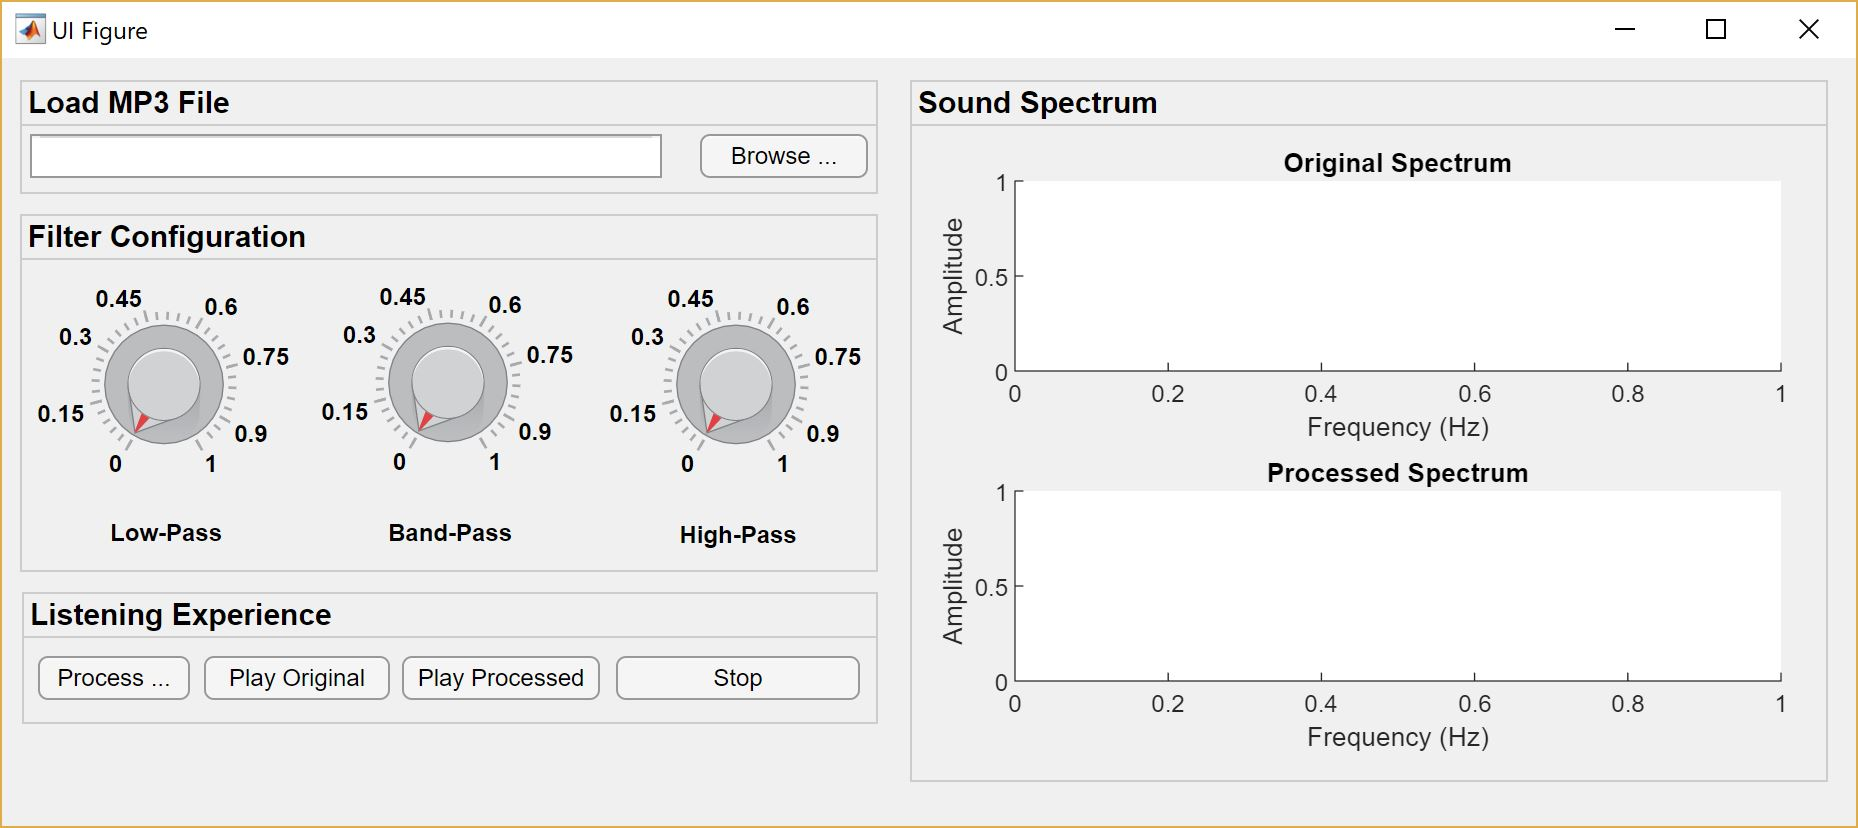
\includegraphics[width=0.65\textwidth]{UIBasic.JPG}
	\end{center}
	\vspace{-1em}
	\caption{Beta-stage user-interface.}
	\label{Beta}
\end{figure}


%
%%---------------------------------------------------------------------------------------------------| ADDITIONAL FEATURES
%

\newpage
\section{Additional Features}

After the basic model had been verified, time remained to add additional features to make our equalizer more useful. In particular, we added the ability for the user to specify their frequency ranges and for the software to generate the appropriate filters based on their choices. Additionally, we decided that the user ought to have the ability to determine what degree of accuracy their filters can achieve so we added the ability to input the filter order, to use higher order filters when more accuracy is necessary. Figure ~\ref{Alpha} illustrates the advanced software in use.

\begin{figure}[h!]
	\begin{center}
		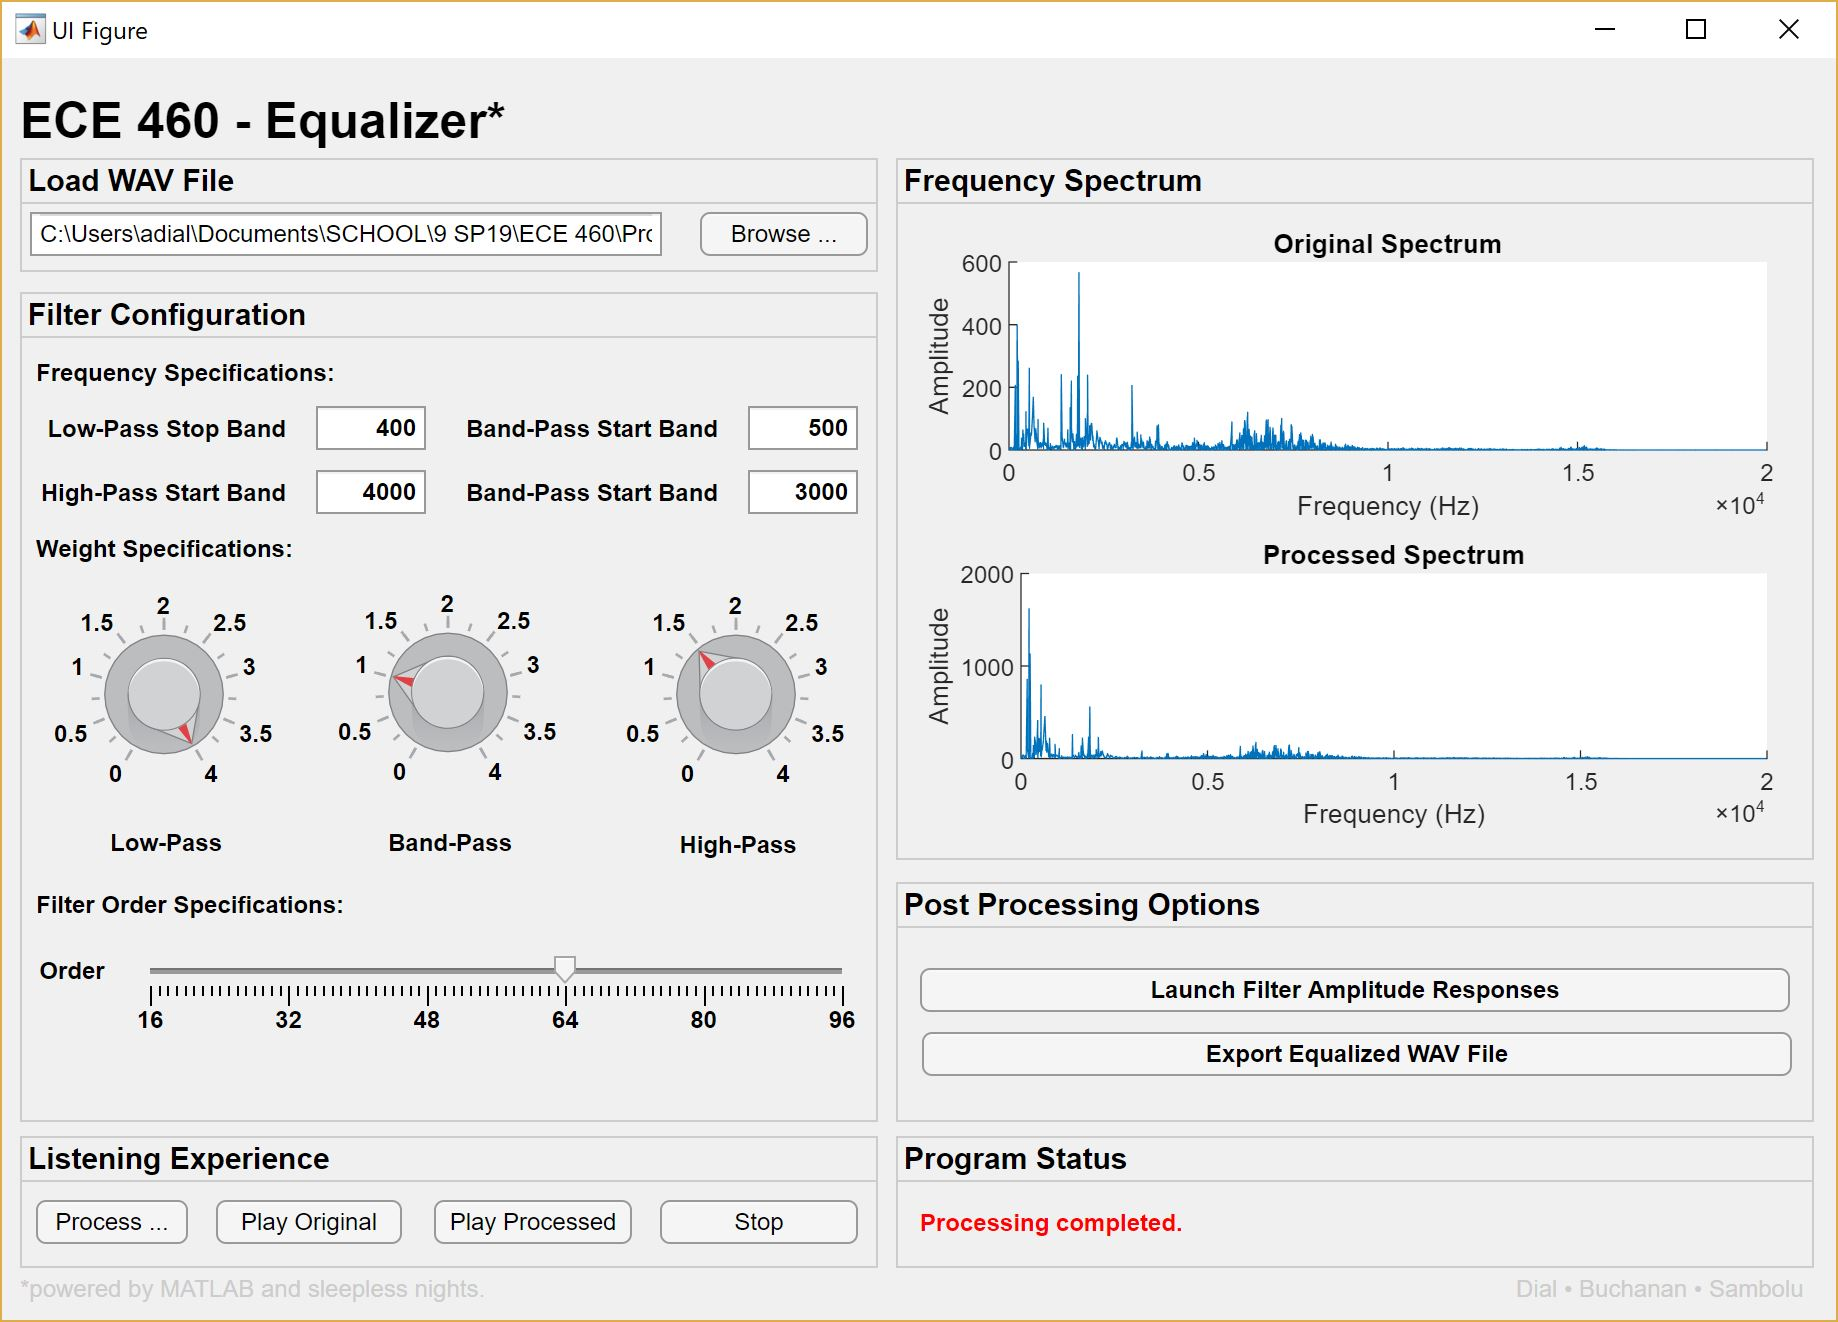
\includegraphics[width=0.65\textwidth]{UIAction.JPG}
	\end{center}
	\vspace{-1em}
	\caption{Advanced user-interface.}
	\label{Alpha}
\end{figure}

\begin{wrapfigure}{r}{0.33\textwidth}
	\begin{center}
		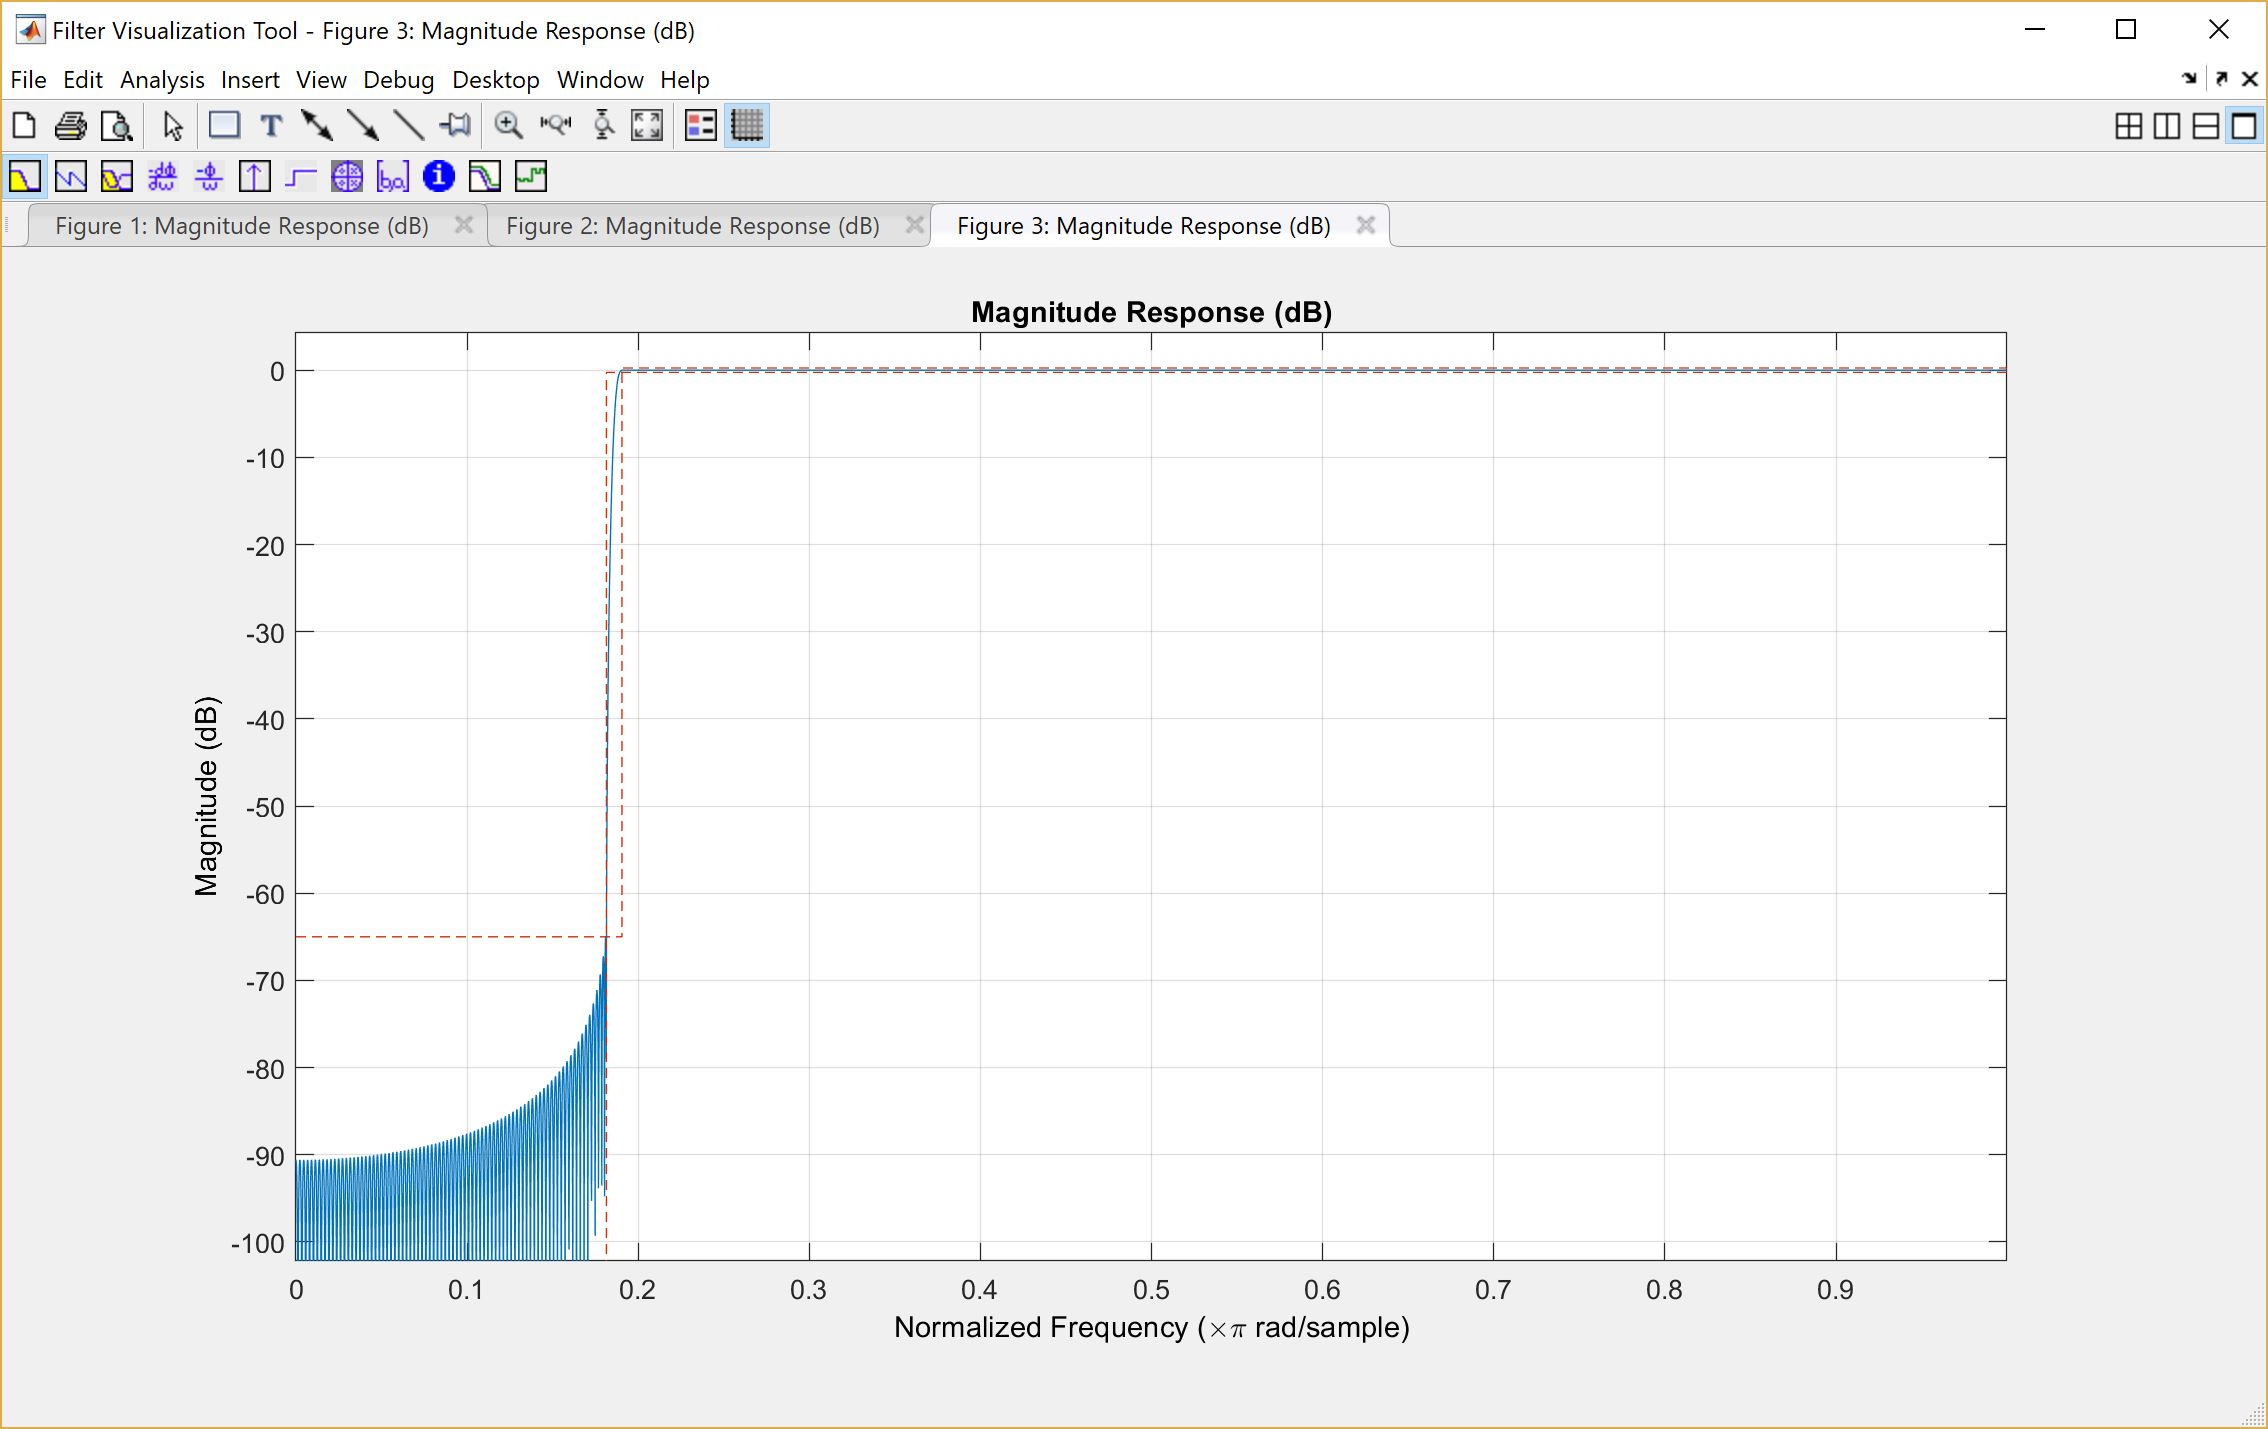
\includegraphics[width=0.32\textwidth]{AmpRes.JPG}
	\end{center}
	\vspace{-1em}
	\caption{Filter amplitude response.}
	\label{FilterView}
\end{wrapfigure}

Once processing is completed, the user ought to be able to retrieve their data, so we added the option to export their equalized audio in the form of a WAV file. If the user is concerned about the accuracy of the filters, they may select the \textit{Launch Filter Amplitude Responses} button to inspect the filters in the MATLAB Filter View, see Figure ~\ref{FilterView}.\footnote{\url{https://www.mathworks.com/help/signal/ref/designfilt.html}} This will inspire confidence that the equalizer is working properly.

Once processing is completed, the user ought to be able to retrieve their data, so we added the option to export their equalized audio in the form of a WAV file. If the user is concerned about the accuracy of the filters, they may select the \textit{Launch Filter Amplitude Responses} button to inspect the filters in the MATLAB Filter View, see Figure ~\ref{FilterView}. This will inspire confidence that the equalizer is working properly.

Lastly, during testing we noticed that high order filters required more time to function properly, so we devised of a program status box which not only directs the user but also informs them when the software is processing and is not ready to take new input. To reinforce this, all buttons become greyed out when the user initializes the processing, this prevents the equalizer from taking conflicting commands during its compute phase. Concordantly, all buttons which cannot logically be used in succession have been programmed to become inaccessible until their use is warranted.



\end{document}

